\documentclass[11pt]{article}
\usepackage{UF_FRED_paper_style}

\usepackage{amsmath,amssymb}
\usepackage{listings}
\usepackage{color}
\definecolor{lightgray}{gray}{0.9}

\lstset{
	showstringspaces=false,
	basicstyle=\ttfamily,
	keywordstyle=\color{blue},
	commentstyle=\color[grey]{0.6},
	stringstyle=\color[RGB]{255,150,75}
}

\newcommand{\inlinecode}[2]{\colorbox{lightgray}{\lstinline[language=#1]$#2$}}

\onehalfspacing
%% ===============================================

\setlength{\droptitle}{-5em} %% Don't touch


% %%%%%%%%%%%%%%%%%%%%%%%%%%%%%%%%%%%%%%%%%%%%%%%%%%%%%%%%%%
% SET THE TITLE
% %%%%%%%%%%%%%%%%%%%%%%%%%%%%%%%%%%%%%%%%%%%%%%%%%%%%%%%%%%

% TITLE:

% ADD UNIPI LOGO

\title{Parallel implementations of a genetic algorithm for the Travelling salesman problem}

% AUTHORS:
\author{Lapo Toloni, 568235 \\% Name author
    \href{l.toloni-at-studenti.unipi.it}{\texttt{l.toloni-at-studenti.unipi.it}}} 

    
% DATE:
\date{\today}

% %%%%%%%%%%%%%%%%%%%%%%%%%%%%%%%%%%%%%%%%%%%%%%%%%%%%%%%%%%
% %%%%%%%%%%%%%%%%%%%%%%%%%%%%%%%%%%%%%%%%%%%%%%%%%%%%%%%%%%
\begin{document}
% %%%%%%%%%%%%%%%%%%%%%%%%%%%%%%%%%%%%%%%%%%%%%%%%%%%%%%%%%%
% %%%%%%%%%%%%%%%%%%%%%%%%%%%%%%%%%%%%%%%%%%%%%%%%%%%%%%%%%%
% ABSTRACT
% %%%%%%%%%%%%%%%%%%%%%%%%%%%%%%%%%%%%%%%%%%%%%%%%%%%%%%%%%%
% %%%%%%%%%%%%%%%%%%%%%%%%%%%%%%%%%%%%%%%%%%%%%%%%%%%%%%%%%%
\maketitle
% %%%%%%%%%%%%%%%%%%

% %%%%%%%%%%%%%%%%%%%%%%%%%%%%%%%%%%%%%%%%%%%%%%%%%%%%%%%%%%
% %%%%%%%%%%%%%%%%%%%%%%%%%%%%%%%%%%%%%%%%%%%%%%%%%%%%%%%%%%
% BODY OF THE DOCUMENT
% %%%%%%%%%%%%%%%%%%%%%%%%%%%%%%%%%%%%%%%%%%%%%%%%%%%%%%%%%%
% %%%%%%%%%%%%%%%%%%%%%%%%%%%%%%%%%%%%%%%%%%%%%%%%%%%%%%%%%%
\section{Problem description} %Algorithmic introduction}
In this report we analyze in theory and in practice the resolution of the famous NP-HARD optimization problem TSP (travelling salesman problem) via a genetic approach.\\
Given a weighted graph $ G=(V,E) $ and its weight function $ w: E \longrightarrow \mathbb{N}$, a solution of TSP is an Hamiltonian tour of $ G $ whose cost is minimum. 
All along this report and in the code we will represent these Hamiltonian tours of $ G $ as permutations $ \rho $ of all the nodes of $ V $  (repetitions are not allowed!). An Hamilton tour of minimum cost is a permutation $ \rho^*$ of $ V $ such that the sum of the weights of successive nodes in $ \rho^* $ is minimal, namely:
\[ \min_{\rho}\ (\sum_{i=0}^{|V|} w(\rho(i),\rho(i+1))) + w(\rho(|V|), \rho(0))  \]
Genetic algorithms are iterative process that aim to find a feasible near-optimal solution to hard optimization problems deploying heuristics that emulate the behaviour of biological systems.\\
Such a complex system is simulated by keeping in memory a collection of chromosomes (i.e. candidate solution) and by trying to improve their fitness value at each iteration. \\
Every genetic algorithm has a common flow that repeats every iteration (usually called generation/epoch in this field's jargon)
\begin{itemize}
	\item $ crossover $: take chromosomes in the current population two-by-two and for every such couple produce two new chromosomes similar to the parents as a result of some combinatorial process.
	\item $ mutate $: take chromosomes in the current population one-by-one and change some part of it.
	\item $ evaluate\ population$: exploit a predefined fitness function to assess how well our population is behaving.
	\item $ selection $: replace ill-fitted chromosomes with copy of the current best ones.
\end{itemize}
Note that both the first two operations above are applied with some given probability for each iteration.

\section{Development of a framework to work with genetic algorithms}
In order to ease the development of a working solution for this project and to be more open to future enhancements we built a tiny framework. The file $ genetic.hpp $ contains a templatic C++ class, named \inlinecode{C++}{Genetic_Algorithm} parametrized by the type of the population, the type of a single chromosome and the type of the used fitness function. \inlinecode{C++}{Genetic_Algorithm} offers a lightweight interface and few protected members to be inherited by its subclasses:
\begin{itemize}
	\item a constructor asking for the maximum number of epochs, the number of chromosomes in the population, the size of a single chromosome and a fitness function.
	\item a function \inlinecode{C++}{void run()} to start the algorithm on the given instance and a function \inlinecode{C++}{get_current_opt()} returning a pair $ (optimum\_value, optimum\_chromosome) $.
	\item four protected functions to obtain the flow presented in the previous section, namely: \inlinecode{C++}{crossover, mutate, eval_population, selection}. These \inlinecode{C++}{void} functions all require as input parameters the start and the end of the range of chromosomes of the population to be deal with by such function calls.
\end{itemize}

\section{Sequential algorithm for genetic TSP}
\subsection{Input graphs}
In order to test the algorithm instead of working on pre-computed graphs that can be scraped from the web, we developed a class \inlinecode{C++}{TSP_Graph}, defined in the header $ tsp\_graph.hpp $ to generate random graphs. Object instances of \inlinecode{C++}{TSP_Graph} are completely connected (each node has an edge to any other node, no self-loops allowed) undirected random weighted graphs. Here the randomness is introduced by the process exploited to assign weights to edges. In fact each edge is given a weight in the interval $ [1,9] $ drawn i.i.d. from a uniform distribution. In memory the graph is stored as an array of adjacency lists that is as a \inlinecode{C++}{std::vector<std::vector<int>> }. Given the properties of the used graph we have an upper triangular matrix that is every element below the diagonal is zero. We did so to spare some time in process of generaing the random graph.

\subsection{Problem representation}
We decided to represent the population of chromosomes as a
\inlinecode{C++}{std::vector<std::vector<int>> } and so the single chromosome as a \inlinecode{C++}{std::vector<int>}. Every element of a chromosome is a natural number $ \in [0, chromosome\_size] $, where the  upper bound $ chromosome\_size $ is one of the parameters used by the constructor of \inlinecode{C++}{Genetic_Algorithm}. $ chromosome\_size $ is also the same parameter defining the size of $ V $ for the \inlinecode{C++}{TSP_Graph} to be generated for this run of the algorithm.

\subsection{Algorithm initialization}
The initialization phase consists in the generation of $ n $ random permutations that will represent the starting population.

\subsection{Crossover}
Many well-refined algorithms to implement crossover functions for genetic TSP can be found in the literature. However we preferred to implement a customize solution. We want to note that the implementation provided does not want to produce better iterates but its main focus is not being too simple and computationally light.\\
The procedure scans the population by rows, two-by-two, and copy the central part of the first chromosome into the central part of the second. Since this procedure may yield candidate solutions that are not feasible (i.e.: chromosomes with repetitions) we apply some sort of sanitization. Through a second linear scan of the two permutations we count numbers appearing twice and we greedly replace them with numbers that never appear in the newly produced children-permutation.

\subsection{Mutate}
It simply consists in a pointwise swap of two elements of a chromosome.

\subsection{Evaluate population}
We scan the matrix representing the population row by row and, using the given fitness function, we compute the cost of the tour represented by that chromosome. Successive elements of a single chromosomes are used as index to access the respective edge weight in the adjacency list of the graph. The fitness value of each chromosome is stored in a vector \inlinecode{C++}{chromosomes_fitness}.

\subsection{Selection}
It consists in a linear scan of the vector \inlinecode{C++}{chromosomes_fitness}. During the scan we keep track of the minimum cost tour and of the maximum cost tour in the current generation. In the end we update the current global optimum tour we found so far. Moreover we inject the current global optimum in the current population in place of the worst chromosome of the current generation.

\subsection{The algorithm as a whole}
We can summarize the algorithm as
\begin{lstlisting}
while current_epoch < max_epoch
  crossover
  mutate
  evaluate_population
  selection
\end{lstlisting}

\section{Parallel solutions design}
Now that all the basic steps that need to be performed by the algorithm were layed down we are able to see from which angle attack the problem. The parallel kind of computation that emerges from this application is the data pallel one.\\
If we look at a single iteration of the algorithm we will see that the subtask of performing a mutation, a crossover and a fitness evaluation on a subgroup of chromosomes is independent from the task of performing the same operations on a different subgroup of chromosomes.\\
Indeed, when we look at the single iteration, the computations here involved are embarassingly parallel. This is implied by the fact that it is just required to split the single-iteration-task: "manipulate the current population and evaluate it" in many equally sized subtasks and then give each subtask to a worker.\\
Note that we are not yet taking into account the $ selection $ part of the algorithm.
If we choose to parallelize this part too we will introduce the classical overhead present in data parallel computations that is the one associated to the time spent in merging the subresults coming from the subtasks. Otherwise by choosing to let a single thread perform all alone the selection task, we introduce some form of "overhead" in the time we have to wait for all the subtasks being completed before starting doing selection. Moreover this single "selecting-worker" will have to deal with a larger chunk of data.
Summarizing, the introduction of parallelism in the implementation of genetic tsp aims to reduce the latency of the task corresponding to a single iteration of the whole genetic algorithm.


\section{Performance modelling}
Having described the sequential version of the algorithm and having presented a tentative design for the parallel implementations, we paved the way to produce some assessment	 about the performances of the model.
\subsection{In theory}
Let $ n = population\_size$ , $m=chromosome\_size$, $ I = max\_epochs $, then we can state:
\[t_{seq} = I * (t_{cro} + t_{mut} + t_{fit} + t_{sel}) \]
where $ t_{cro}$, $ t_{mut}$, $t_{fit}$, $t_{sel}$ are respectively the time spent in performing crossovers, mutations, population evaluations and selections. Then we bound time complexities of the steps of the algorithm as:
\\ \medskip
\begin{itemize}
	\item $ t_{cro} \approx \mathcal{O}(m) * \mathcal{O}(n) \approx \mathcal{O}(m*n) $
	\item $ t_{mut} \approx \mathcal{O}(1) * \mathcal{O}(n) \approx \mathcal{O}(n) $
	\item $ t_{fit} \approx \mathcal{O}(m) * \mathcal{O}(n) \approx \mathcal{O}(m*n) $
	\item $ t_{sel} \approx \mathcal{O}(n)$
\end{itemize}
Glueing pieces together, we obtain
\begin{align*}
t_{seq} &= I * (t_{cro} + t_{mut} + t_{fit} + t_{sel}) \\
& \approx I * ((\mathcal{O}(m*n) + \mathcal{O}(n) + \mathcal{O}(m*n)) + \mathcal{O}(n))\\
& \approx I * (\mathcal{O}(m*n) + \mathcal{O}(n)) \\
& \approx I * \mathcal{O}(m*n) \approx \mathcal{O}(m*n)\\
\end{align*}
With the last $ \approx $ coming from the fact that $ I $ is usually orders of magnitude less then both $ m $ and $ n $. \\
Recalling that we will deploy parallelism only for crossovers, mutations and evaluation,
what we are trying to enlight with this reasoning is that even if we chose to not parallelize the selection phase the performance loss should remain negligible since its computational complexity is cancelled by the complexity of the three previous tasks.

\subsubsection{Ideal Parallel performances}
Following everything we stated so far about
\begin{itemize}
  \item the points from where the problem of parallelizing our sequential algorithm can be attacked;
  \item  $ t_{cro}$, $ t_{mut}$, $t_{fit}$, $t_{sel}$ theoretical time complexities;
\end{itemize} 
Then, assuming that $ p $ is the number of workers at disposal for our parallel computation, we can define the ideal parallel time:
\[ t_{par\_ideal} = \frac{t_{seq}}{p} \]
and we will use it as benchmark for our experimental results.\\
We define the ideal $ speedup $, the ideal $ scalability $ and the ideal efficiency using the definition of such measures and our definition of $ t_{par\_ideal} $:
\begin{align*}
s(p) = \frac{t_{seq}}{t_{par}(p)} = \frac{t_{seq}}{t_{seq}/p} = p 
&
& scalab(p) = \frac{t_{par}(1)}{t_{par}} = \frac{t_{seq}/1}{t_{seq}/p} = p 
&
& \varepsilon(p) = \frac{t_{seq}}{p*t_{par}(p)} = \frac{t_{seq}}{p*t_{seq}/p} = 1 
\end{align*}

\subsection{In practice.. Overheads}
A world where these ideal assumptions hold is just an utopy. Indeed we know both from theory and real life cases that parallel computations comes with overheads. To defend our choices of what to and what to not parallelize we measured the time taken by each step of an iteration of the algorithm in the sequential version:
\begin{table}[h]
	\begin{center}
	  \begin{tabular}{||c | c | c | c||}
	  \multicolumn{4}{||c||}{Sequential implementation} \\ \hline
	  $ t\_cro $ & $ t\_mut $  & $t\_fit$ & $t\_sel $  \\ \hline
	  165143&265&1480653&15 \\ \hline
	  \end{tabular}
	\captionof{table}{Results of a sequential run on an instance with $ max\_epochs =10 $, $ population\_size=1024 $, $chromosome\_size=10000$. Reported times are in microseconds and each number is an average of 10 runs.} 
	\end{center}
\end{table}

Since forking/joining a single thread takes a fraction of time in the range [500, 800] microseconds (CPU Xeon Phi KNC, 64 physical cores), it would not be convenient to a adopt a parallel solution and so the choice we made seems exact.



\section{Parallel implementations: structure and details}
We provide three parallel implementations of the algorithm. Each one is implemented in C++17. Two rely on native C++ threads while the third one exploits the FastFlow framework. The implementations are thought to avoid race conditions between workers dealing with different parts of the algorithm data. This let us avoid the explicit use of locks and any other special synchronization mechanism except for the ones hidden behind the FastFlow front-end and the one used to manage the \inlinecode{C++}{condition_variable} used in the task queue exploited by the thread pool.\\
Each implementation is available as an .hpp header file in the directory ./include.
The directory ./src contains .cpp files that are the drivers of the relative .hpp files.
To compile the project is enough to run the bash script $ compile.sh $ located in the root of the project folder. To run a default batch of experiments use the bash script $ run.sh $. More details on the directory structure of the project and on how to play with this piece of software can be find in $ README.md $ file.

\subsection{Naive C++ thread implementation}
Both the native c++ thread implementations realize a Map parallel pattern exploting the embarassingly parallel kind of computation that emerges from a single iterations subtask. These subtasks can be shaped as: $  evaluate \circ mutate \circ crossover (population) $. \\
We could also look at the $ selection $ function as a Reduction even if in these two versions we preferred to leave this last task to a single worker and so any merge of subresults comes out. The only point in the program that needs a form of synchronization is the one preceeding the selection since we may need some kind of barrier to not let the main thread start the $ selection $ before every worker did not yet finish its subtask. Since every thread is joined just after having finished its task an implicit form of barrier comes out from the sequence of joins that are called and so no more code is needed.\\
The two c++ threads implementations differ only on how they manage the workers' threads. 
The first and most naive one just add an \inlinecode{C++}{std::vector<thread>} as a class field and use it in the function that simulates a single iteration of the genetic algorithm, namely \inlinecode{C++}{next_generation()}. This function forks a thread for each worker and joins again these threads after they have completed their tasks. This becomes even worse since the series of forks/joins repeats three times every iteration of the whole algorithm. This naive implementation never uses two twice the same thread and indeed it loses much time in spawning new dumb threads only capable of performing one specific task.

\subsection{Thread pool C++ implementation}
This implementation still realizes a Map-like computation but uses smartly its workers. Instead of using one-time-use threads it makes use of a thread pool that mantains a queue of tasks to be polled from a defined number of thread. These threads are created once at the beginning of the computation and never joined before its end. Moreover these smarter workers are not limited to perform only one specific task being more versatile. The pool implementation uses \inlinecode{C++}{std::future} and \inlinecode{C++}{std::condition_variable} to synchronize and manage its threads.

\subsection{FastFlow implementation}
The implementation grounded on FastFlow realizes the algorithm with a Master-Workers farm. To meet the design requirements we defined two FastFlow nodes:
\begin{itemize}
	\item \inlinecode{C++}{TSP_Master : ff::ff_monode_t<TSP_Task >} is a node that emits and collects \inlinecode{C++}{TSP_Task} where such a task is an helper struct that encapsulated the range of rows of the population matrix on which the receiver worker will work on and a collection of \inlinecode{C++}{std::shared_ptr<>} to the data structures of the algorithm. The master node deals with task dispatching when nothing comes in its input channels, and it deals with $ selection $ when it is sure he collected all the sent tasks of the current generation.
	\item \inlinecode{C++}{TSP_Worker : ff::ffnode_t<TSP_Task >} is a node that receives tasks from the master, performs $evaluate \circ mutate \circ crossover (population)$, sends back its results and goes to sleep waiting for a new task dispatched by the master.
\end{itemize} 
It is worthy to note that all the implementations does not perform copies of the data they work with. Different concurrent entities communicate and share data via smart pointers and move semantics.

\section{Experimental validation}
\subsection{Experiments details}
The experiments have been executed on a CPU Xeon Phi KNC with 64 physical cores, each of them with a four-way multithreading support. In particular
\begin{itemize}
	\item each completion time is expressed in microseconds and it is an average of 10 repeated runs on instances of the same size
	\item each parallel implementation was tested with parallel degree p $ \in [2^{0}, 2^{1}, 2^{2}, \dots , 2^{8}] $
	\item the reported results are runs of the algorithm on problem sized:
	\begin{itemize}
		\item 10 $ max\_epochs $;
		\item 1024 $chromosomes$;
		\item 10000 nodes in the graph ($chromosome\_size$);
	\end{itemize}
\end{itemize}

\subsection{Completion time}
As a first result we report in a table the completion times achieved by each provided implementation.
\begin{table}[h]
	\begin{center}
		\begin{tabular}{|l|r|r|r|r|r|r|r|r|r|}
			\cline{2-10} 
			\multicolumn{1}{c|}{} & \multicolumn{9}{ c| }{$p$} \\ \hline
			Impl.& $2^{0}$  & $2^{1}$ & $2^{2}$ & $2^{3}$ & $2^{4}$  & $2^{5}$ & $2^{6}$ & $2^{7}$& $2^{8}$ \\ \hline
			\hline
			seq  & 16911497 & -       & -       &  -      &  -       &  -      & -       & -      & -      \\ \hline
			\hline
			par  & 15293248 & 7900973 & 3671931 & 1788209 &  953265  &  630667 &  592633 & 808949 & 1171651 \\ \hline 
			pool & 15145325 & 7750127 & 4015389 & 2145586 &  1326911 &  895351 &  476426 & 294825 & 386614 \\ \hline
			ff   & 16579772 & 8773667 & 4331534 & 2103021 &  1074172 &  589713 &  476579 & 420941 & 786272 \\ \hline
			\hline
			ideal& 16911497 & 8455748 & 4227874 & 2113937 &  1056968 &  528484 &  264242 & 132121 & 66060  \\ \hline
		\end{tabular}
	\end{center}
\end{table}
\smallskip
From this first glimpse to raw data we can already see how completion time of the parallel naive implementation is the lowest up to a parallel degree of 16. After that the noise produced by such a large quantity of repeated creations and destructions of threads makes it underperforming. Viceversa the thread pool implementation takes a while to gain traction but in the end for the two highest tested parallel degrees (128, 256) it peaks among the other implementations. Last but not least, FastFlow implementation shines for parallel degrees near and equal to the maximum number of physical cores of the testing machine (32, 64) and so it seems to suffer of excess parallelism/parallel slack.\\
However the most important experimental fact to note is that experiments'results are in line with the ideal performance model up to a parallel degree of 32. After that point the costs of the overheads introduced to manage all the concurrent activities are no more negligible.

\subsection{Plots of performance measures}
We now plot the obtained result to give a clearer idea of the performances of our implementations.

\begin{center}
	\begin{minipage}{\textwidth}
		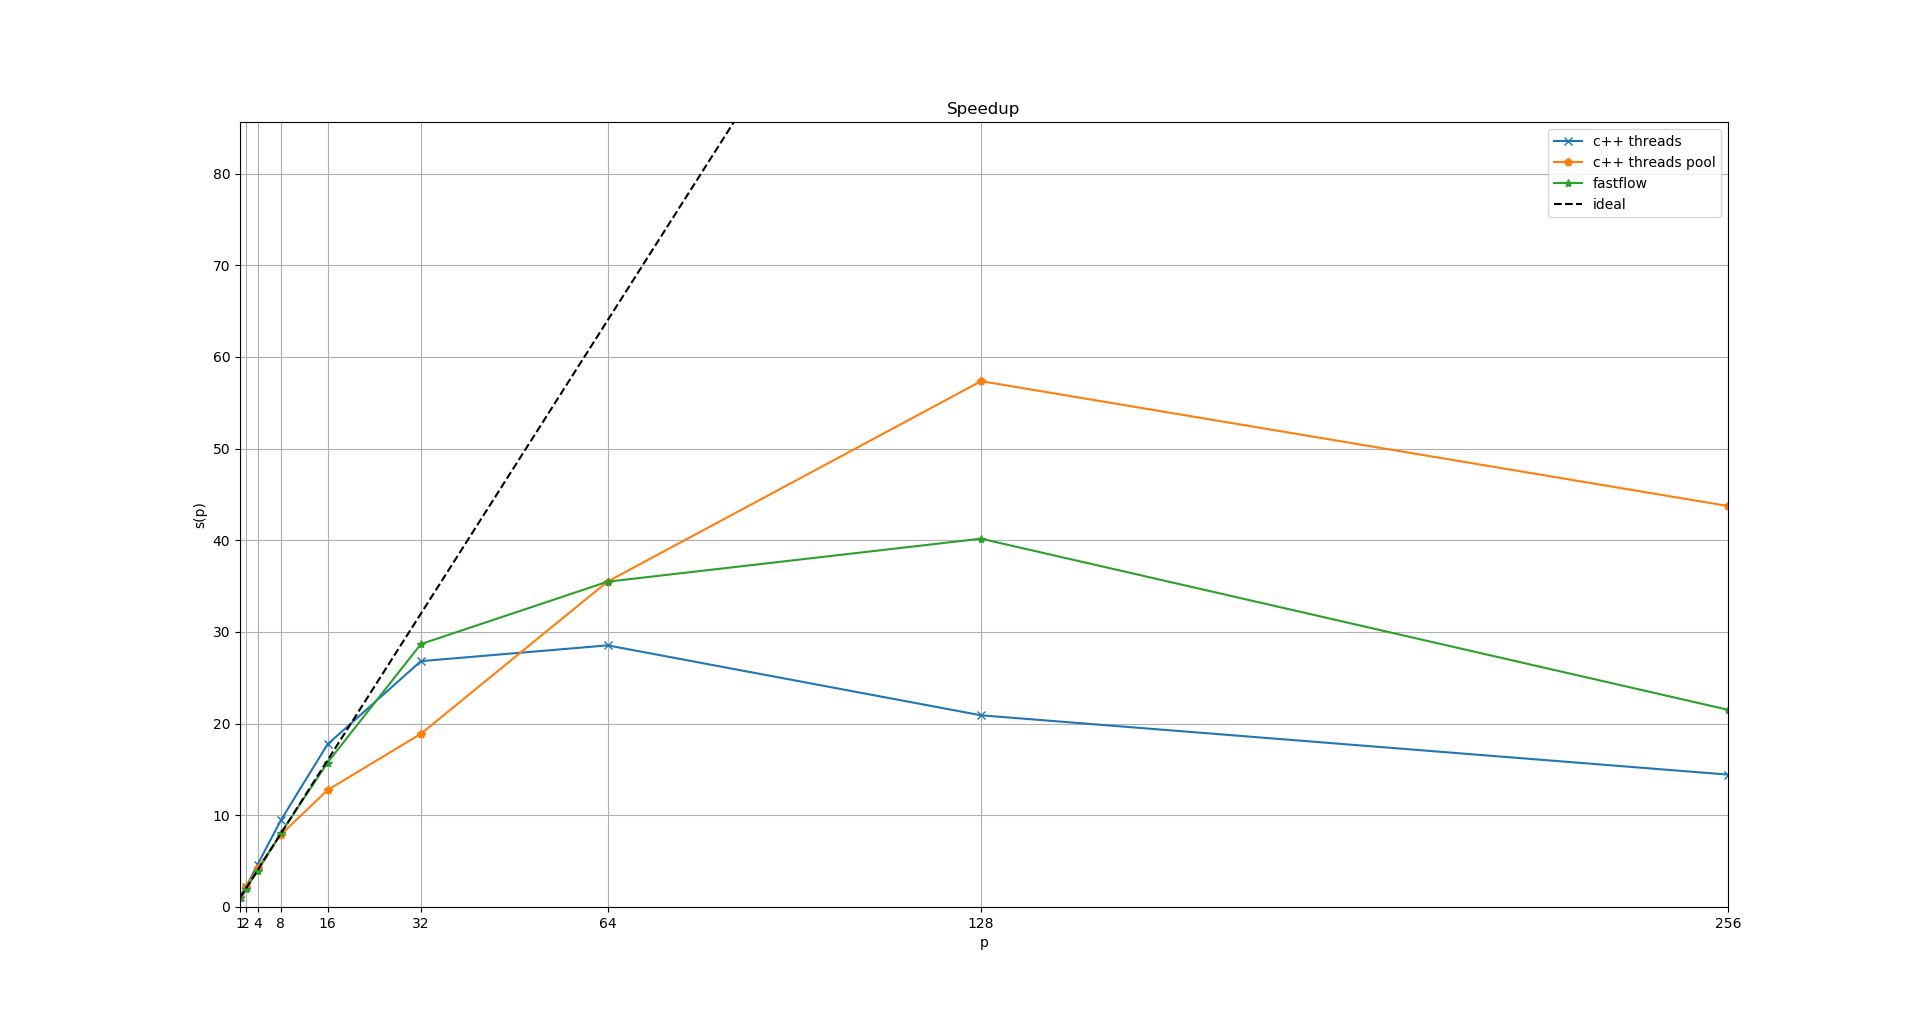
\includegraphics[width=\linewidth]{plots/SPEEDUP-10-1024-10000.png}
		\captionof{figure}{$s(p)$ of each implementation, $max\_epochs=10$, $population\_size=1024$, $chromosome\_size=10000$} 
	\end{minipage}
\end{center}
The plot shows us that the thread pool implementation has the best speedup overall when the parallel degree becomes high. The FastFlow version instead is the closest to the ideal model for $ p \in [1,32] $. The naive implementation follows the FastFlow implementation up to $ p=32 $. Then it suddenly worsen because of its bad thread management. \\



\begin{center}
	\begin{minipage}{\linewidth}
		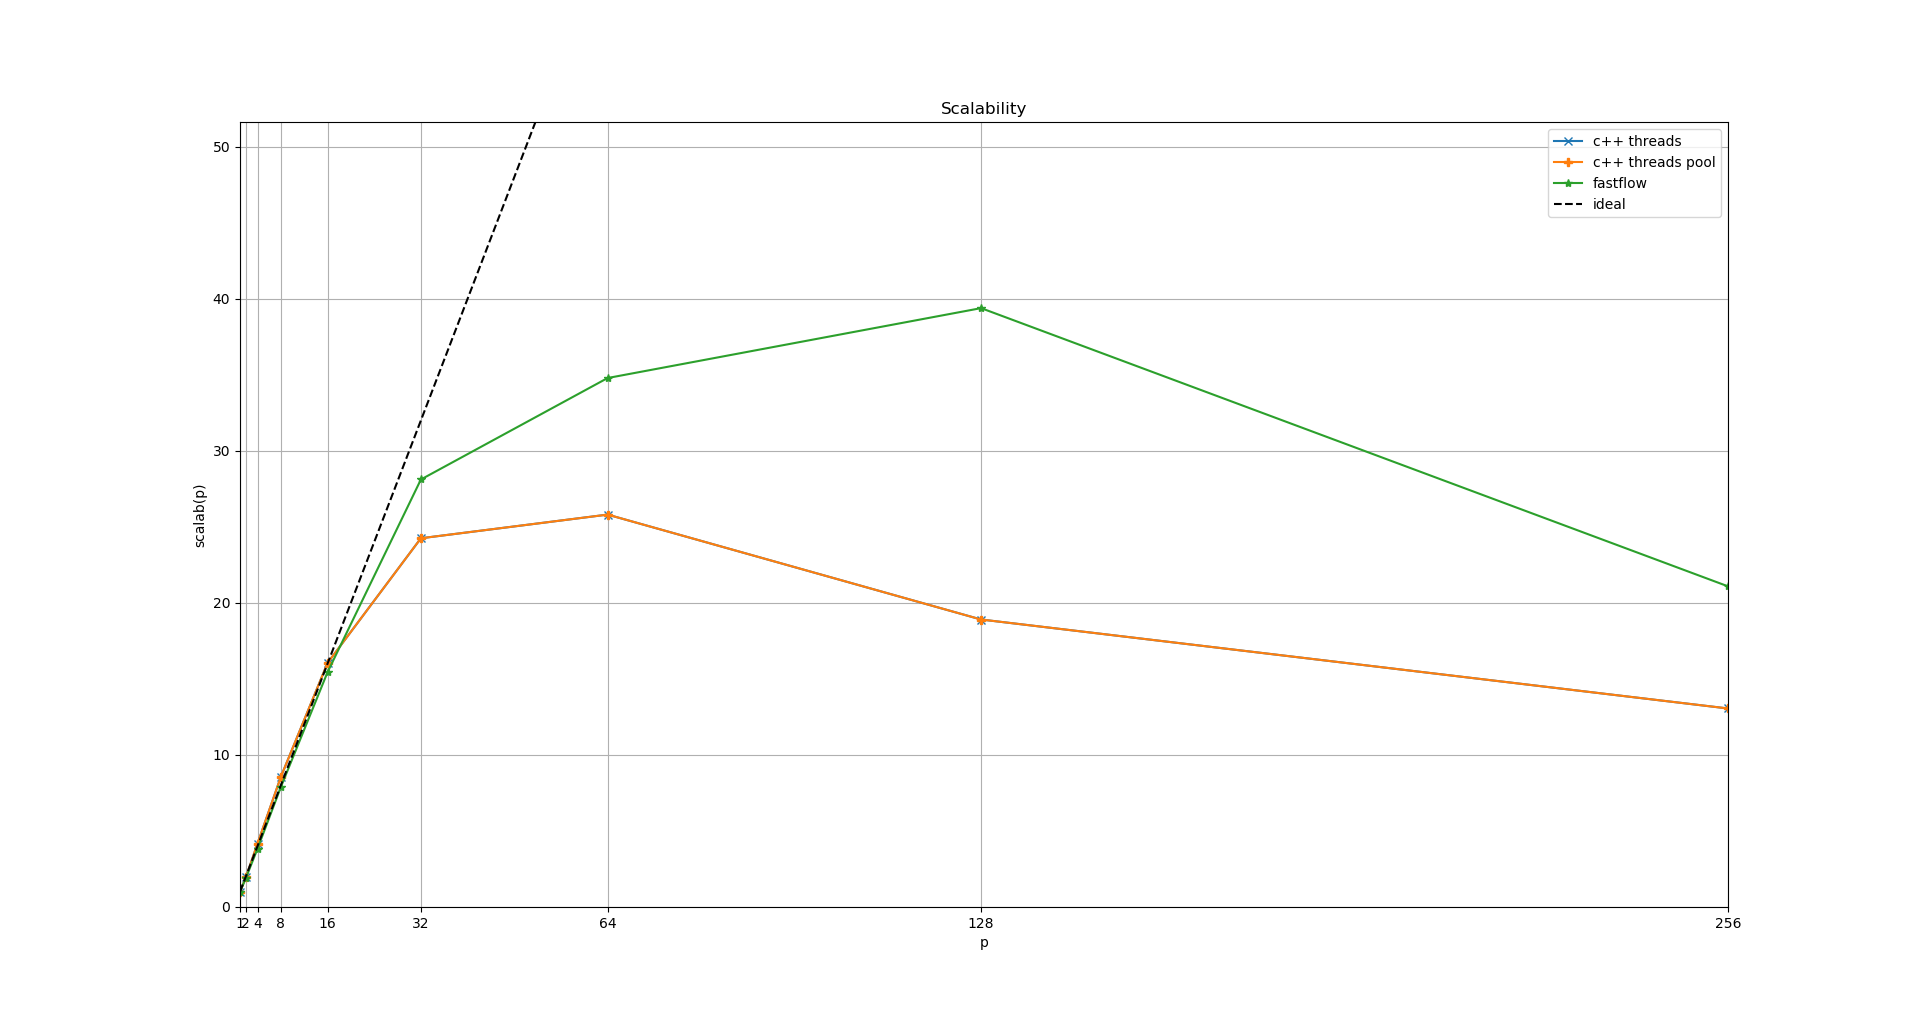
\includegraphics[width=\linewidth]{plots/SCALAB-10-1024-10000.png}
		\captionof{figure}{$scalab(p)$ of each implementation, $max\_epochs=10$, $population\_size=1024$, $chromosome\_size=10000$} 
	\end{minipage}
\end{center}
Here the plot confirms what we previously observed in the data regarding completion times.
Naive implementation scales well only with a few number of computing cores. FastFlow follows the ideal scalability up to 32 cores, then it keeps on scale but on a line that is almost flat. Instead the thread pool implementation after a starting section that is the less scaling it reveals to outscale the other two.


\begin{center}
	\begin{minipage}{\linewidth}
		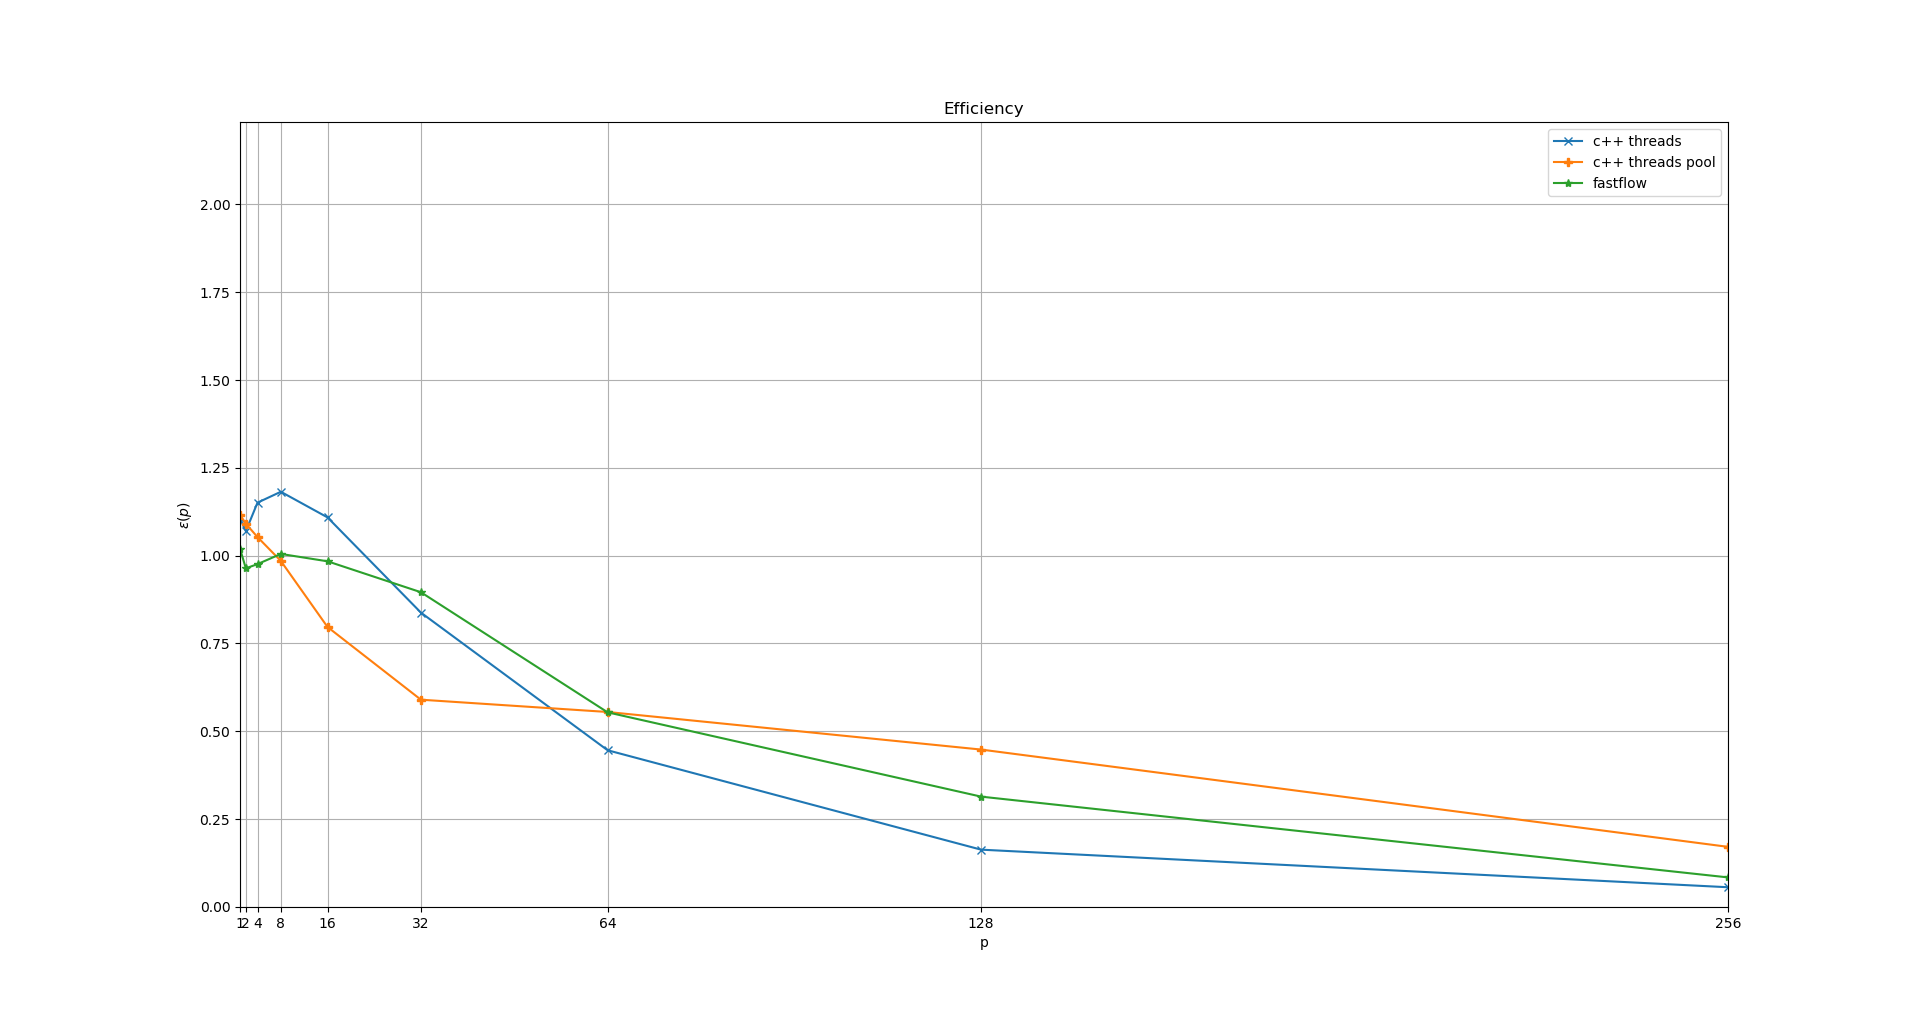
\includegraphics[width=\linewidth]{plots/EFFI-10-1024-10000.png}
		\captionof{figure}{$\varepsilon(p)$ of each implementation, $max\_epochs=10$, $population\_size=1024$, $chromosome\_size=10000$} 
	\end{minipage}
\end{center}
Regarding efficiency we can see that the naive version is the most efficient for low values of $ p $ up to $ p=32 $. In the interval $ [32, 64] $ FastFlow dominates but in the next interval the thread pool implementation becomes the best one.

\begin{center}

\end{center}

\begin{center}

\end{center}


\end{document}